\section{OPC-UA}
\label{sec:opcua}

Eine Kommunikation mittels HTTPS und REST, mit Daten in Form von JSON oder XML funktioniert gut für eine Umgebung wie das Internet und mit Endgeräten wie Web-Browsern, sowie Web-Servern auf der Serverseite. Doch während diese Art der Kommunikation der de-facto Standard für das Internet ist, hat sie sich nicht für die Kommunikation für Technologien im Umfeld von Industrie 4.0 etabliert. In diesem Umfeld ist Interoperabilität zwischen Hardware, Software und Diensten verschiedener Hersteller nicht nur außerordentlich wichtig, sondern bisherige Technologien wie Web-Browser oder Web-Server sind auch unnötig komplex.\\
Open Platform Communications (OPC), beziehungsweise spezifischer OPC Unified Architecture (OPC-UA), ist daher ein offener Standard, welcher speziell für solche Anwendungen entworfen wurde und von verschiedenen Branchenanbietern weiterentwickelt und erweitert wird [\cite{opcua}]. Neben der Offenheit und der kollaborativen Natur des Standards bietet OPC-UA auch noch andere Vorteile, wie ein erweiterbares, umfangreiches Datenmodell. Dieses Datenmodell lässt sich leicht in neue Technologien und Methoden integrieren, während es gleichzeitig mit älteren Produkten kompatibel bleibt. Ein weiterer zentraler Punkt und ein wichtiges Anliegen von OPC-UA ist Sicherheit, welche tief in den Standard integriert ist. Neben offensichtlichen Eigenschaften wie Verschlüsselung sind daher auch Aspekte wie Authentifizierung, Autorisierung, und Zugriffskontrollen eingebettet.\\
OPC-UA ist dabei ein neuerer Standard aus der OPC Familie. Wie der Name andeutet, ist der wesentliche Fokus von OPC-UA, eine einheitliche Architektur zu ermöglichen, welche eine größtmögliche Kompatibilität besitzt. In dieser Arbeit liegt der Fokus daher vollkommen auf OPC-UA, weshalb OPC und OPC-UA im folgenden als austauschbar zu verstehen sind.

In der OPC Architektur gibt es – wie auch im herkömmlichen Internet üblich – immer Server und Clients. Der OPC-Server ist dabei ein Softwareprogramm, welches eine Schnittstelle zur verwendeten Hardware bildet. Es wird also meist ein von einer Speicherprogrammierbaren Steuerung (SPS, engl.: Programmable Logic Controller, PLC) verwendetes Hardware-Kommunikationsprotokoll in das OPC-Protokoll umgewandelt. In der Regel hat jede Steuerungseinheit einen OPC-Server, und üblicherweise ist dieser auch direkt Teil der SPS. Grafik \ref{fig:OPC} bildet ein solches OPC-UA Netzwerk ab.
%
\begin{figure}[htbp]
	\centering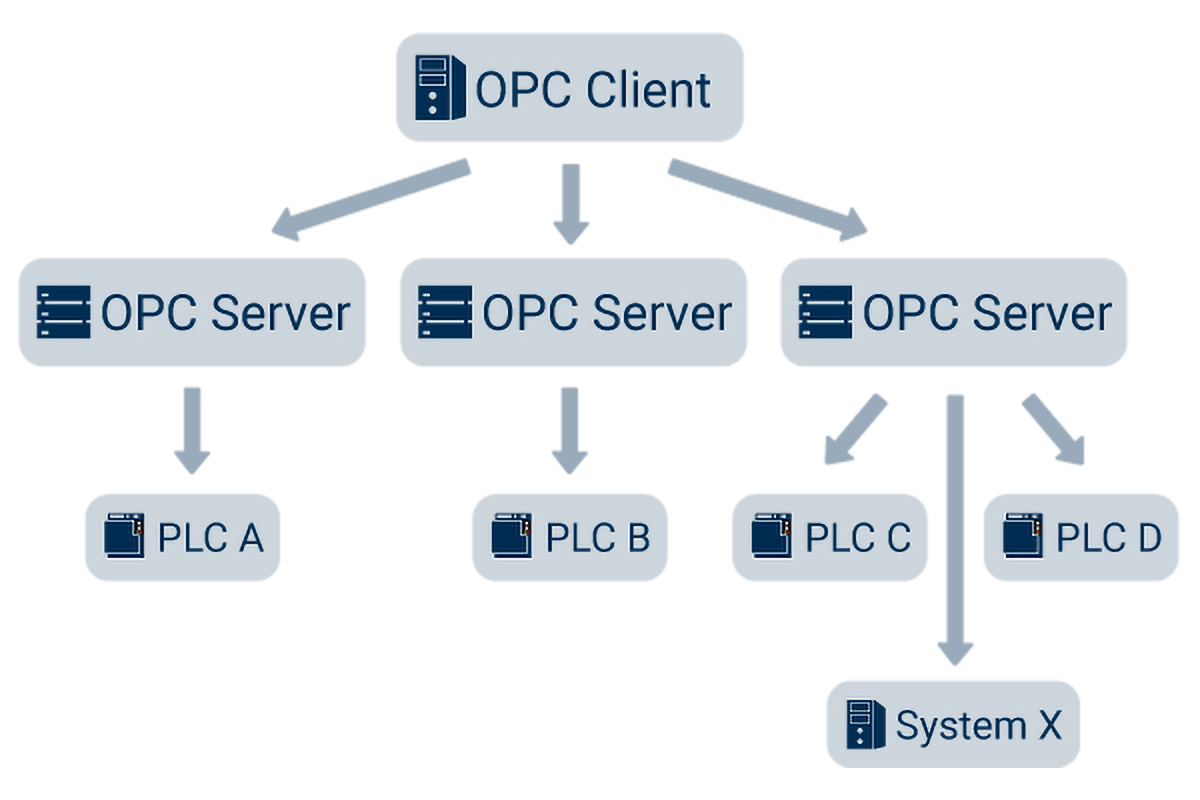
\includegraphics[width=0.7\textwidth]{images/03/OPC_Netzwerk.png}
    \caption{OPC-UA Netzwerk [\cite{opcNetwork}]}
    \label{fig:OPC}
\end{figure}

OPC-UA Datenmodelle basieren auf Graphen, welche wiederum aus Knoten und Referenzen bestehen. Es gibt acht standardisierte Knotenklassen, welche die Attribute sowie die Semantik des Knotens definieren. Innerhalb eines Graphen können dabei sowohl die strukturellen Aspekte als auch die dynamischen Zusammenhänge eines Systems dargestellt werden [\cite{opcAnderl}].

\subsection*{Vergleich zu REST APIs}
\label{subsec:opcua_vergleichrest}

Zunächst sei gesagt, dass OPC-UA und REST APIs nicht direkt verglichen werden können, da sie einen leicht unterschiedlichen Umfang haben. OPC-UA ist wesentlich spezieller als eine REST API, bei welcher es darum geht, wie Daten im weiteren Sinne ausgetauscht werden. Bei OPC-UA dagegen sind Mechanismen wie Pub/Sub (Publish/Subscribe), Filterung, Ereignisse, Alarme, historische Daten, usw. schon eingebunden und müssen nicht separat implementiert werden. Es sollte bei einem Vergleich also berücksichtigt werden, dass solche Methoden – sofern benötigt – bei einem Softwaresystem, welches auf einer REST API basiert, noch auf anderem Wege hinzugefügt werden müssen.

Streng genommen ist OPC-UA nicht zustandslos, da zum Aufbau eines sicheren Kanals zur Kommunikation eine Art Zustand gespeichert wird, aber wenn über dieses Implementierungsdetail hinweggesehen wird, kann OPC-UA als praktisch zustandslos bezeichnet werden. Dazu sollte auch gesagt sein, dass eine REST API auf das gleiche Problem stoßen kann, wenn es darum geht, eine sichere Kommunikation zwischen dem Server und Client aufzubauen, allerdings ist dies dort nicht in den Standard eingebettet und kann daher auch anders gelöst werden.

Tabelle \ref{tab:opcVsRest} vergleicht OPC-UA und REST APIs in einigen Punkten grob miteinander, um Gemeinsamkeiten und Unterschiede aufzuzeigen. Manche dieser Punkte sind dabei bewusst verallgemeinert, wie etwa die Tatsache, dass nicht absolut alle PLCs einen integrierten OPC-Server haben. Der Punkt „TCP-basiert“ verweist hier darauf, dass beide Arten der Kommunikation über TCP/IP funktionieren. Das bedeutet, dass zwar der Mehraufwand von TCP dazu kommt, aber das wird in den meisten Fällen von den Vorteilen aufgewogen, an erster Stelle der Absicherung vor verlorenen oder korrumpierten Datenpaketen. Bei einer REST API ist eine Kommunikation über User Datagram Protocol (UDP) daher nicht möglich, da die üblichen HTTP Protokolle (z.B. GET, POST, PATCH, etc.) schlichtweg über TCP funktionieren. Bei OPC-UA allerdings ist diese Einschränkung nicht gegeben, und es kann auch über UDP kommuniziert werden. Dies ist üblicherweise nicht der Standard, aber es kann zu Verbesserungen führen, wenn exemplarisch große Datenmengen gestreamt werden müssen und Datenverlust nicht allzu relevant ist. Zur Verschlüsselung sei gesagt, dass auf beide Arten eine Verschlüsselung möglich und zum aktuellen Stand der Technik auch der Standard ist, aber es ist dennoch nicht ausgeschlossen, Daten auch unverschlüsselt zu übertragen (im Falle einer REST API etwa via HTTP statt über HTTPS). Bei beiden Kommunikationsarten findet die Verschlüsselung gleichwertig statt.\\
Im Gegensatz zu ASCII-Dateien, die über RESTful-Architekturen gesendet werden, bietet OPC-UA ein umfassenderes Gerätedatenmodell und Datenwerte, die ihren ursprünglichen Datentyp, Genauigkeit und Korrektheit beibehalten [\cite{whyOpc}].
%
\bgroup
\def\arraystretch{1.5}
\vspace{5mm}\begin{table}[htbp]
    \centering
    \begin{tabularx}{140mm}{@{}p{80mm}|*3{>{\centering\arraybackslash}X}@{}}
        \rowcolor{dikblue} \mbox{\color{white}\textbf{}} & \mbox{\color{white}\textbf{OPC-UA}} & \mbox{\color{white}\textbf{REST API}} \\
        Benutzbar über Web-Browser & \FeatureFalse & \FeatureTrue \\ \hline
        Integriert in PLCs & \FeatureTrue & selten \\ \hline
        Pub/Sub & \FeatureTrue & \FeatureFalse \\ \hline
        TCP-basiert & (\FeatureTrue) & \FeatureTrue \\ \hline
        Verschlüsselte Übertragung & (\FeatureTrue) & (\FeatureTrue)\\ \hline
        Betriebssystemübergreifend & \FeatureTrue & \FeatureTrue
    \end{tabularx}
    \caption{Vergleich zwischen OPC-UA und REST APIs}
    \label{tab:opcVsRest}
\end{table}
\egroup

In Tabelle \ref{tab:httpAndUpc} werden die HTTP Methoden, welche von einer REST API benutzt werden, zu ihren äquivalenten OPC-UA Diensten und den dazugehörigen MIME-Typ eingeordnet. Die Tabelle umfasst dabei natürlich nur einige der abstrakten Dienste von OPC-UA, doch sie gibt eine Vorstellung darüber, wie Entsprechungen zwischen OPC-UA und einer REST API aussehen.
%
\bgroup
\def\arraystretch{1.5}
\vspace{5mm}\begin{table}[htbp]
    \centering
    \begin{tabularx}{140mm}{@{\hspace{2mm}}p{18mm}|@{\hspace{2mm}}p{32mm}|@{\hspace{2mm}}X@{}}
        \rowcolor{dikblue} \mbox{\color{white}\textbf{HTTP}} \newline \mbox{\color{white}\textbf{Methode}} & \mbox{\color{white}\textbf{OPC-UA}} \newline \mbox{\color{white}\textbf{Dienste}} & \mbox{\color{white}\textbf{MIME-Typ}} \newline \mbox{\color{white}\textbf{Repräsentation}} \\
        GET & Read & app/opcua.Boolean+json \newline app/pdf \newline … \\ \hline
        GET & HistoryRead & app/opcua.HistoryReadResult+json \\ \hline
        PUT & Write & app/opcua.Boolean+json \newline app/pdf \newline … \\ \hline
        PATCH & HistoryUpdate & app/opcua.HistoryUpdateResult+json \newline app/json-patch+json \\ \hline
        GET & Browse & app/opcua.NodeRepresentation+json \\ \hline
        GET & BrowseNext & app/opcua.NodeRepresentation+json \\ \hline
        GET & TranslateBrowse & app/opcua.BrowsePathResult+json \newline PathsToNodeIds \\ \hline
        POST & Call & app/opcua.CallRequest+json \newline app/opcua.CallResult+json \\ \hline
        POST & AddNode & app/opcua.CallRequest+json \newline app/opcua.CallResult+json \\ \hline
        DELETE & DeleteNode & app/opcua.StatusCode+json \\ \hline
        POST & Query & app/opcua.CallRequest+json \newline app/opcua.CallResult+json \\ \hline
        GET & QueryNext & app/opcua.QueryNextResponse+json
    \end{tabularx}
    \caption{HTTP Methoden und äquivalente OPC-UA Dienste [\cite{restBasedIiot}]}
    \label{tab:httpAndUpc}
\end{table}
\egroup

Abschließend lässt sich also zusammenfassen, dass OPC-UA eingebaute Sicherheitsfunktionen, flexiblere Transportmechanismen, Codierungen, Dienste und Datenmodellierungsfunktionen zur Verfügung stellt, während REST APIs zwar unkompliziert und einfach sind, dies aber auf Kosten der Funktionalität geht.\\
Es sollte sich also vor Augen geführt werden, dass beide Architekturen ihre Stärken in verschiedenen Richtungen haben und sie meist nicht in direkter Konkurrenz zueinander stehen. In vielen Fällen ist es sogar wünschenswert oder erforderlich, beides zu kombinieren. So ist es etwa möglich, eine über den Browser erreichbare REST API zu entwickeln, welche über eine Middleware mit einem OPC-Server direkt auf einer PLC kommuniziert.
